%%%%%%%%%%%%%%%%%%%%%%%%%%%%%%%%%%%%%%%%%
% Professional Mathematical Presentation Template
% 
% This template uses the beamer class with the Madrid theme
% and a custom color scheme for a clean, professional look
% that works well with mathematical content.
%%%%%%%%%%%%%%%%%%%%%%%%%%%%%%%%%%%%%%%%%
\documentclass[aspectratio=169]{beamer} % 16:9 aspect ratio (modern)
% Theme settings
\usetheme{Madrid}
\usecolortheme{default}
\usepackage[dvipsnames]{xcolor}
\definecolor{primcolor}{RGB}{25,50,100} % Dark blue
\setbeamercolor{structure}{fg=primcolor}
\setbeamercolor{frametitle}{bg=primcolor!15, fg=primcolor}
\setbeamercolor{title}{fg=white} % White title text for contrast
\setbeamercolor{subtitle}{fg=white} % White subtitle text
\setbeamercolor{author}{fg=primcolor} % White author text
\setbeamercolor{date}{fg=primcolor} % White date text
\setbeamercolor{institute}{fg=primcolor} % White institute text
% Font settings
\usefonttheme{professionalfonts}
\usefonttheme{serif}
% Package imports
\usepackage{amsmath, amsfonts, amssymb, amsthm} % Math packages
\usepackage{mathtools} % Enhanced math tools
\usepackage{bm} % Bold math symbols
\usepackage{graphicx} % For images
\usepackage{booktabs} % Professional tables
\usepackage{tikz} % For diagrams
\usetikzlibrary{arrows, positioning, matrix, decorations.pathreplacing}
% Use beamer's theorem styles
\setbeamertemplate{theorem}[ams style]
\setbeamertemplate{theorems}[numbered]
% Remove navigation symbols
\setbeamertemplate{navigation symbols}{}
% Custom footer
\setbeamertemplate{footline}{
  \leavevmode%
  \hbox{%
  \begin{beamercolorbox}[wd=.333333\paperwidth,ht=2.25ex,dp=1ex,center]{author in head/foot}%
    \usebeamerfont{author in head/foot}\insertshortauthor
  \end{beamercolorbox}%
  \begin{beamercolorbox}[wd=.333333\paperwidth,ht=2.25ex,dp=1ex,center]{title in head/foot}%
    \usebeamerfont{title in head/foot}\insertshorttitle
  \end{beamercolorbox}%
  \begin{beamercolorbox}[wd=.333333\paperwidth,ht=2.25ex,dp=1ex,right]{date in head/foot}%
    \usebeamerfont{date in head/foot}\insertshortdate{}\hspace{2em}
    \insertframenumber{} / \inserttotalframenumber\hspace{2ex} 
  \end{beamercolorbox}}%
  \vskip0pt%
}
% Title information
\title[DP2]{Dynamic Programming}
\subtitle{Thomas J. Sargent and John Stachurski}
\author[Longye]{Longye Tian \\ \texttt{longye.tian@anu.edu.au}}
\institute[ANU]{Australian National University\\ School of Economics}
\date{May 2nd, 2025}
\DeclareFontFamily{U}{mathx}{\hyphenchar\font45}
\DeclareFontShape{U}{mathx}{m}{n}{
      <5> <6> <7> <8> <9> <10>
      <10.95> <12> <14.4> <17.28> <20.74> <24.88>
      mathx10
      }{}
\DeclareSymbolFont{mathx}{U}{mathx}{m}{n}
\DeclareMathSymbol{\bigtimes}{1}{mathx}{"91}

\begin{document}

% Title frame
\begin{frame}
  \titlepage
\end{frame}

% Outline frame

\begin{frame}{Setup}
\begin{itemize}
    \item \textbf{Wage space}: $\mathbf{W}\in [0,M]\subset \mathbb{R}_+$ and $M>0$.
    \item \textbf{Wage offer}: $(W_t)$ is $P$-Markov on $\mathbf{W}$.
    \item \textbf{State space}: $\mathbf{X} = \{e,u\}\times \mathbf{W}$, $e\implies$ employed; $u\implies$ unemployed
    \item \textbf{Policy}: a Borel measurable map: $\sigma: \mathbf{X}\to \{0,1\}$, i.e., we only choose when unemployed
    \item \textbf{Separation probability} $:= \alpha $, the probability of job termination
\end{itemize}
    
\end{frame}


\begin{frame}{ADP with Job Search with Separation}
    \begin{itemize}
        \item \textbf{Value space}: $\mathbf{V} = bm(\mathbf{X}, \mathbb{R})$ with supremum norm and pointwise partial order
        \item \textbf{Policy operator when employed} (let $v_u:= v(u,\cdot); \quad v_e:=v(e,\cdot);\quad \mathbf{w}(w):= w$, and $\mathbf{c}(w) := c$)
        $$
        T_\sigma v_e= \mathbf{w}+\beta\left[\underbrace{\alpha Pv_u}_{\text{transit to unemployed }} + \underbrace{(1-\alpha) v_e}_{\text{stay employed}}\right]
        $$
        \textbf{Remark}: we don't have $\sigma$ explicitly here.
        \item \textbf{Policy operator when unemployed}
        $$
        T_\sigma v_u = \underbrace{\sigma v_e}_{\text{transit to employed}} + \underbrace{(1-\sigma)\left[\mathbf{c}+\beta Pv_u\right]}_{\text{stay unemployed}}
        $$
    \end{itemize}
\end{frame}

\begin{frame}{Simplify}
    We treat the policy operator when employed as a fixed point problem i.e.,
    $$
    T_\sigma v_e= \mathbf{w}+\beta\left[\alpha Pv_u + (1-\alpha) v_e\right]
    $$
    to
    \begin{align*}
        v_e &= \mathbf{w}+\beta\left[\alpha Pv_u + (1-\alpha) v_e\right]\\
        &= \mathbf{w} + \alpha\beta Pv_u + \beta(1-\alpha) v_e\\
        &= \frac{1}{1-\beta(1-\alpha)}[\mathbf{w}+ \alpha\beta Pv_u]\\
        &= \underbrace{\frac{1}{1-\beta(1-\alpha)}\mathbf{w}}_{=:\mathbf{h}} + \underbrace{\frac{\alpha\beta}{1-\beta(1-\alpha)}}_{=:\gamma}Pv_u\\
        v_e&= \mathbf{h}+ \gamma Pv_u\tag{a relation between $v_e$ and $v_u$}
    \end{align*}
\end{frame}
\begin{frame}{Reduce dimension}
For the policy operator when unemployed:
    $$
    T_\sigma v_u = \sigma v_e + (1-\sigma)\left[\mathbf{c}+\beta Pv_u\right]
    $$
    we have $v_e = \mathbf{h} + \gamma P v_u$, then, we have
    $$
    T_\sigma v_u = \sigma(\mathbf{h}+\gamma Pv_u) + (1-\sigma) [\mathbf{c} + \beta P v_u]
    $$
    now we reduce the state space into just $\mathbf{W}$ compared to $\mathbf{X}= \{e,u\}\times \mathbf{W}$.
\end{frame}
\begin{frame}{Reduce dimension}
The state space is reduced from $\mathbf{X}=\{e,u\}\times \mathbf{W}$ to $\mathbf{W}$, we can reduce the value space
$$
\mathbf{V} = bm(\mathbf{X},\mathbb{R}) \text{  to  $bm(\mathbf{W},\mathbb{R})=: bm\mathbf{W}$}
$$
with policy operator
$$
T_\sigma v_u = \sigma(\mathbf{h}+\gamma Pv_u) + (1-\sigma) [\mathbf{c} + \beta P v_u]
$$
\textbf{Remark}: We can rewrite $T_\sigma v_u = s_\sigma + K_\sigma v_u$, where $s_\sigma  = \sigma \mathbf{h} + (1-\sigma)\mathbf{c}$; and $K_\sigma  = (\sigma \gamma +(1-\sigma) \beta))P$
\end{frame}

\begin{frame}{Prove that $T_\sigma$ is an order preserving self-map on $bm\mathbf{W}$}
\begin{proof}[Proof of order preserving]
Fix $\sigma\in\Sigma$. Let $v_u^1\le v_u^2\in bm\mathbf{W}$, For $w\in \{w\in \mathbf{W}: \sigma(w) =1\}$, we have
$$
T_\sigma v_u^1(w) = h(w)+\gamma (Pv_u^1)(w) \le h(w) + \gamma (Pv_u^2)(w)
$$
by order preserving of the Markov operator $P$. For $w'\in \{w\in \mathbf{W}: \sigma(w)=0\}$, we have
$$
T_\sigma v_u^1(w) = c + \beta (Pv_u^1)(w')\le c+\beta(Pv_u^2)(w')
$$
by order preserving of the Markov operator $P$. Hence in all, we have
$$
T_\sigma v_u^1\le T_\sigma v_u^2
$$
Hence, $T_\sigma$ is order preserving.
\end{proof}
    
\end{frame}

\begin{frame}{Prove that $T_\sigma$ is an order preserving self-map on $bm\mathbf{W}$}
\begin{proof}[Proof of $T_\sigma v_u$ is bounded]
   Fix $\sigma\in\Sigma$:
    \begin{align*}
        \|T_\sigma v_u\|_\infty &= \|(\sigma \mathbf{h}+(1-\sigma )\mathbf{c}) + (\sigma \gamma+(1-\sigma)\beta)Pv_u\|_\infty\\
        &\le \|\sigma \mathbf{h}+(1-\sigma )\mathbf{c}\|_\infty + \|(\sigma \gamma+(1-\sigma)\beta)Pv_u\|_\infty \tag{$\Delta$ ineq.}\\
        &\le \|\mathbf{h}\|_\infty +\|\mathbf{c}\|_\infty  + (\gamma+\beta)\|Pv\|_\infty \tag{$\Delta$ ineq.}\\
        &\le \frac{M}{1-\beta(1-\alpha)} + c+ (\gamma+\beta)\|v\|_\infty\tag{$\|P\|=1$}\\
    \end{align*}
\end{proof}
\textbf{Remark}: another way to bound $\|(\sigma \gamma+(1-\sigma)\beta)Pv_u\|_\infty\le \lambda \|v\|_\infty$, $\lambda:=\max\{\gamma,\beta\}$
\end{frame}

\begin{frame}{Prove that $T_\sigma$ is an order preserving self-map on $bm\mathbf{W}$}
    \begin{proof}[Proof of $T_\sigma v_u$ is Borel measurable]
        \begin{itemize}
            \item $v_u$ is Borel measurable
            \item $P$ is bounded linear operator hence continuous hence Borel measurable
            \item $\sigma$ is Borel measurable
            \item $\mathbf{h}$, $\mathbf{c}$ are constant functions hence Borel measurable.
        \end{itemize}
        Hence, $T_\sigma v_u$ is Borel measurable.
    \end{proof}
    Hence, we have $(bm\mathbf{W}, \mathbb{T})$, $\mathbb{T}:=\{T_\sigma: \sigma\in\Sigma\}$ is an ADP (still $bm\mathbf{W}$ has a \textcolor{blue}{supremum norm} and pointwise partial order).
\end{frame}
\begin{frame}{Why supremum norm?}
\textbf{Claim 1: The metric induced by supremum norm is sup-nonexpansive.}\\
Let $(v_n), (w_n)\in bm\mathbf{W}$ with supremum $v$ and $w$ which are bounded above. We have
\begin{align*}
    v_n &= v_n-w_n+w_n\\
    &\le |v_n-w_n|+w_n\\
    &\implies\\
    \sup_n v_n&\le \sup_n(|v_n-w_n|+w_n)\le \sup_n|v_n-w_n|+\sup_n w_n\\
    \sup_n v_n - \sup_nw_n&\le \sup_n|v_n-w_n|
\end{align*}
Similar for the other direction, we have
$$
|\sup_n v_n-\sup_nw_n|\le \sup_n|v_n-w_n|
$$
    
\end{frame}
\begin{frame}{Supremum norm induce a sup-nonexpansive metric}
For 
$$
|\sup_n v_n-\sup_nw_n|\le \sup_n|v_n-w_n|
$$
we have
$$
\sup_{x\in \mathbf{W}} |\sup_n v_n(x)-\sup_nw_n(x)|\le \sup_{x\in \mathbf{W}} \sup_n|v_n(x)-w_n(x)|= \sup_n\sup_{x\in \mathbf{W}}|v_n(x)-w_n(x)|
$$
the last equality is by the uniquness of supremum. This implies
$$
\|\sup_n v_n - \sup_n w_n\|_\infty \le \sup_n\|v_n-w_n\|_\infty
$$
in term of the metric induced by supremum norm, we have
$$
d_\infty(\sup_n v_n, \sup_n w_n)\le \sup_n d_\infty(v_n,w_n)
$$
Hence, supremum norm induce a \textcolor{blue}{sup-nonexpansive metric}
    
\end{frame}
\begin{frame}{Why supremum norm?}
\textbf{Claim 2: The metric induced by supremum norm is complete.}\\
Let $(v_n)$ be a Cauchy sequence in $bm\mathbf{W}$. By definition, for any $\varepsilon>0$, there exists $N\in \mathbb{N}$ such that for all $m,n\ge N$, we have
$$
d_\infty (v_m,v_n) = \sup_{x\in \mathbf{W}}|v_m(x)-v_n(x)|<\varepsilon
$$
This implies for a fixed $x\in \mathbf{W}$, $(v_n(x))$ is a Cauchy sequence in $\mathbb{R}$ (with Euclidean metric). By the completeness of $\mathbb{R}$, we get there exists $v$ such that
$$
v(x) = \lim_{n\to\infty }v_n(x)
$$
Now we just need to show that $v\in bm\mathbf{W}$ and $d_\infty(v_n,v)<\epsilon$.
\end{frame}
\begin{frame}{Supremum metric is complete}
\textbf{Measurability}: For $v_n:\mathbf{W}\to\mathbb{R}$, pointwise limit of measurable function is measurable. (See details in appendix page \ref{app:pointwise})\\
\textbf{Boundedness}: let $m,n\ge N$, we have
$$
|v_m(x) - v_n(x)|<\epsilon \implies |v_m(x)|\le |v_m(x)-v_n(x)|+|v_n(x)|<\epsilon + |v_n(x)|
$$
for all $m\ge N$, hence
$$
\lim_{m\to\infty}|v_m(x)| = |v(x)|<\epsilon +|v_n(x)|
$$
hence bounded.
\end{frame}
\begin{frame}{Supremum metric is complete}
    \textbf{Convergence in supremum metric}:
    $$
    \sup_{x\in \mathbf{W}}|v_n(x)-v_m(x)|<\epsilon,\forall m\ge N
    $$
    implies
    $$
    \sup_{x\in \mathbf{W}} |v_n(x)-v(x)| <\epsilon 
    $$
    Hence, $d_\infty$ is a \textcolor{blue}{complete} metric. This makes the underlying value space $(bm\mathbf{W},\|\cdot\|_\infty)$ a \textcolor{blue}{Banach space}.
\end{frame}
\begin{frame}{$v_u$-greedy policy}
    Claim: $\sigma(w):= \mathbf{1}\{v_e(w)\ge c+\beta (Pv_u)(w)\}$ is $v_u$-greedy
    \begin{proof}
    Note under $\sigma$, we have
    $$
    T_\sigma v_u = \max\{v_e , c+\beta Pv_u\}
    $$
        Fix $\tau\in \Sigma$, we have
        $$
        T_\tau v_u = \tau(v_e) + (1-\tau)(c+\beta Pv_u) \le \max\{v_e, c+\beta Pv_u\} = T_\sigma v_u
        $$
    Hence, $\sigma$ is $v_u$-greedy
    \end{proof}
    \textbf{Remark 1}: economic interpretation is choose the one with higher expected discounted payoff.\\
    \textbf{Remark 2}: Since for every $v_u$, such greedy policy is well-defined as above, we have the ADP is \textcolor{blue}{regular}
\end{frame}
\begin{frame}{Exercise 4.2.10}
Prove that there exists $\lambda\in (0,1)$ such that $T_\sigma$ is a contraction of modulus $\lambda$ on $bm\mathbf{W}$ for all $\sigma\in\Sigma$.
\begin{proof}
Recall that we can rewrite $T_\sigma v_u = s_\sigma + K_\sigma v_u$, where $s_\sigma  = \sigma \mathbf{h} + (1-\sigma)\mathbf{c}$; and $K_\sigma  = (\sigma \gamma +(1-\sigma) \beta))P$. 
    Let $v_1,v_2\in bm\mathbf{W}$. We have
    \begin{align*}
        \|T_\sigma v_1-T_\sigma v_2\|_\infty  &=  \|s_\sigma + K_\sigma v_1- (s_\sigma+K_\sigma v_2)\|_\infty\\
        &= \|K_\sigma (v_1-v_2)\|_\infty\tag{$K_\sigma$ is linear}\\
        &= \|(\sigma \gamma +(1-\sigma)\beta)P (v_1-v_2)\|_\infty\\
        &\le \|\lambda P(v_1-v_2)\|_\infty\tag{$\lambda:=\max\{\gamma,\beta\}\in(0,1)$}\\
        &\le \lambda \|v_1-v_2\|_\infty\tag{$\|P\|=1$}
    \end{align*}
\end{proof}
\end{frame}
\begin{frame}{Remark and Summary}
\textbf{Remark}: As shown before, the value space is a Banach space. Hence, by the Banach fixed point theorem, every policy operator has a unique fixed point and globally stable. And the ADP is well-posed.\\
\textbf{Summary}: Now we know that the 
\begin{itemize}
    \item ADP is \textcolor{blue}{regular} and well-posed.
    \item Supremum norm induces a \textcolor{blue}{complete and sup-nonexpansive metric}
    \item Every policy operator is a \textcolor{blue}{contraction}, globally stable with unique fixed point
\end{itemize}
\end{frame}
\begin{frame}{Proposition 4.2.2. Optimality}
        The ADP $(bm\mathbf{W}, \mathbb{T})$ is well-posed. Moreover
        \begin{enumerate}
            \item the fundamental optimality properties hold, and
            \item VFI, OPI and HPI all converge
        \end{enumerate}
    \begin{proof}
        Invoke Theorem 1.3.5. See next page
    \end{proof}
\end{frame}
\begin{frame}{Theorem 1.3.5}
    \begin{figure}
        \centering
        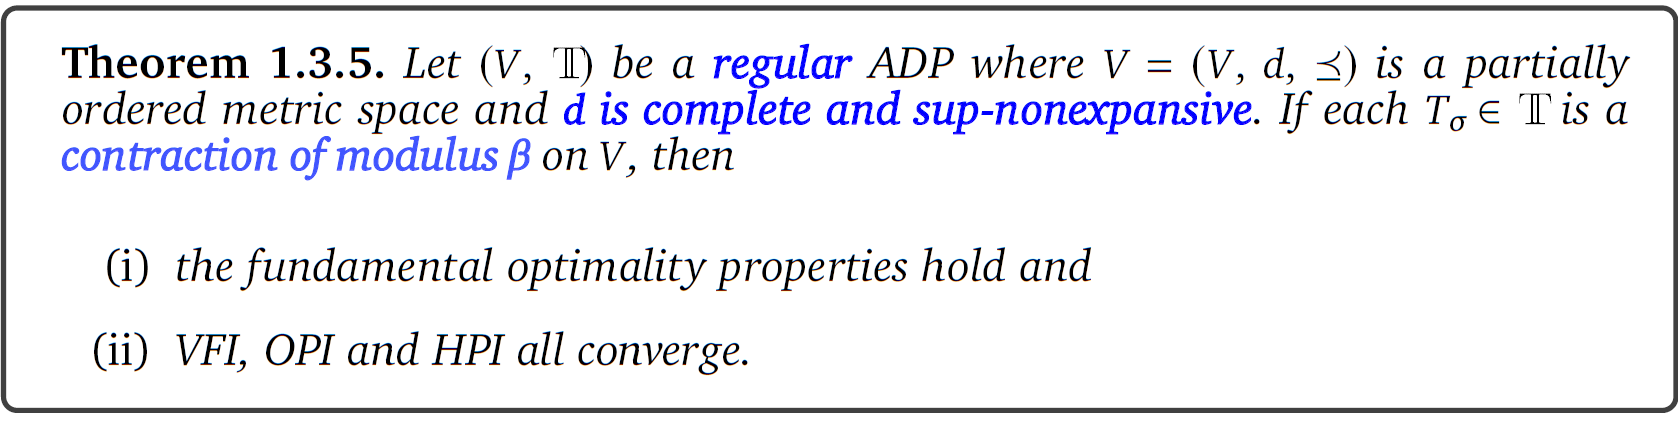
\includegraphics[width=1\linewidth]{Dynamic Programming/DP2/Chapter 4/4.2.4.1 Job Search with Separation/thm135.png}
    \end{figure}
\end{frame}
\begin{frame}{Appendix 1 - pointwise limit}\label{app:pointwise}
    Let 
    \begin{itemize}
        \item $(\mathbf{X},\mathcal{A})$ be a measurable space
        \item $(f_n)$ be a sequence of measurable functions from $\mathbf{X}$ to $\mathbb{R}$
        \item $f(x) = \lim_{n\to\infty} f_n(x)$
    \end{itemize}
    By definition, $f$ is measurable if
    $$
    f^{-1}((-\infty, \alpha])\in\mathcal{A},\quad \forall \alpha\in\mathbb{R}
    $$
    i.e., we need to show $\{x\in \mathbf{X}: f(x)\le \alpha\}$ is measurable. 
\end{frame}

\begin{frame}{Appendix 1 - pointwise limit}
Using the definition of limit we have,
\begin{align*}
    \{x\in \mathbf{X}: f(x)\le \alpha\} &= \{x\in \mathbf{X}: \forall\epsilon>0,\exists N\in\mathbb{N}, \forall n\ge N, f_n(x)<\alpha+\epsilon\}\\
    &= \bigcap_{\epsilon>0}\bigcup_{N\in\mathbb{N}}\bigcap_{n\ge N} \{x\in \mathbf{X}: f_n(x)<\alpha+\epsilon\}\\
    &= \bigcap_{\epsilon>0,\epsilon\in \mathbb{Q}}\bigcup_{N\in\mathbb{N}}\bigcap_{n\ge N}\underbrace{\{x\in \mathbf{X}: f_n(x)<\alpha+\epsilon\}}_{\text{measurable}}\tag{$\mathbb{Q}$ is dense in $\mathbb{R}$}\\
\end{align*}
Hence $\{x\in \mathbf{X}: f(x)\le \alpha\}$ is a countable intersection of countable union of countable intersection of measurable set, hence measurable.
    
\end{frame}

\begin{frame}{Appendix 2 - Optimal policy}
Let $\sigma^\top$ be the optimal policy and $v_u^\top$ be the value function. We have
$$
v_u^\top = \max\{h+\gamma Pv_u^\top, c\mathbf{1} + \beta Pv_u^\top\}
$$
We can define optimal stopping value
$$
s^\top = h+\gamma Pv_u^\top
$$
and 
optimal continuation value
$$
f^\top = c\mathbf{1}+\beta Pv_u^\top
$$
Hence, we can characterize the optimal policy as
$$
\sigma^\top = \mathbf{1}{\{s^\top\ge f^\top\}}
$$
\end{frame}
\begin{frame}{Appendix 2 - Reservation wage}
We define the smallest $w\in W$ such that $\sigma^\top (w) =1$ as \textbf{reservation wage}.
    
\end{frame}
\end{document}
